\documentclass[11pt,addpoints]{exam}
\usepackage{amsfonts,amssymb,amsmath, amsthm}
\usepackage{graphicx}
\usepackage{systeme}
\usepackage{pgf,tikz,pgfplots}
\pgfplotsset{compat=1.15}
\usepgfplotslibrary{fillbetween}
\usepackage{mathrsfs}
\usetikzlibrary{arrows}
\usetikzlibrary{calc}
\usepackage{enumitem}
\usepackage{multicol}

\pagestyle{headandfoot}
\firstpageheader{AP Calc. AB - Exam 3 Practice Problems\\ Exam date: September 7}{}{Name: \underline{\hspace{2.5in}}}
\runningheader{AP Calc. AB - Exam 3 Practice Problems}{}{Page \thepage\ of \numpages}
\runningheadrule
\firstpagefooter{}{}{}
\runningfooter{}{}{}
\begin{document}
\begin{questions}
\question Using the table above, evaluate the following: % TODO: Try and move the table below?
\begin{table}[]
	\begin{tabular}{|l|l|l|l|l|l|l|}
		\hline
		x$\quad$$\quad$ & $\quad$1$\quad$ & $\quad$2$\quad$ & $\quad$3$\quad$ & $\quad$4$\quad$ & $\quad$5$\quad$ & $\quad$6$\quad$ \\ \hline
		$f(x)$          & $\quad$2$\quad$ & $\quad$4$\quad$ & $\quad$4$\quad$ & $\quad$6$\quad$ & $\quad$3$\quad$ & $\quad$1$\quad$ \\ \hline
		$g(x)$          & $\quad$1$\quad$ & $\quad$1$\quad$ & $\quad$1$\quad$ & $\quad$5$\quad$ & $\quad$2$\quad$ & $\quad$5$\quad$ \\ \hline
		$h(x)$          & $\quad$4$\quad$ & $\quad$4$\quad$ & $\quad$3$\quad$ & $\quad$1$\quad$ & $\quad$2$\quad$ & $\quad$2$\quad$ \\ \hline
	\end{tabular}
\end{table}
\begin{multicols}{2}
	\begin{parts}
		\part $f(h(f(1)))\div (f\circ g)(2)$
		\part $(h\circ g \circ f)(5)$
		\part $g(f(3))-h(h(2))$
		\part $(f\circ g)(h(f(4)))$
	\end{parts}
\end{multicols}


\question From the graphs of $f$, $g$, and $h$ below, estimate the values of $g(f(h(x))$ for $\{x\hspace{0.125cm}\epsilon\hspace{0.125cm}\mathbb{Z} \mid -3\leq x\leq 3\}$. % TODO: Add the graph...
\begin{center}
	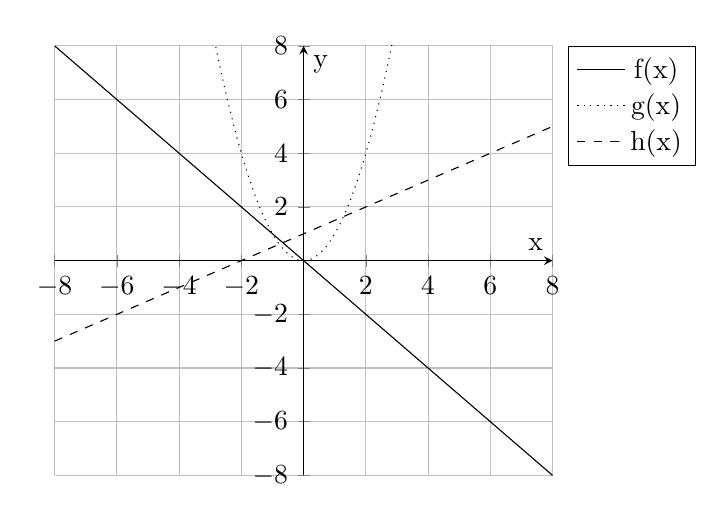
\begin{tikzpicture}
		\begin{axis}
			[
				xlabel={x},
				ylabel={y},
				grid,
				scale only axis,
				xmin=-8,
				xmax=8,
				ymin=-8,
				ymax=8,
				xtick={-8,-6,...,8},
				ytick={-8,-6,...,8},
				axis lines=center,
				legend pos=outer north east,
				tick align=center,
				scale=0.75
			]
			\addplot[no marks, smooth, domain=-8:8, samples=50] {-x};
			\addlegendentry{f(x)}
			\addplot[no marks, smooth, dotted, domain=-8:8, samples=50] {x^2};
			\addlegendentry{g(x)}
			\addplot[no marks, smooth, dashed, domain=-8:8, samples=50] {x/2+1};
			\addlegendentry{h(x)}

		\end{axis}
	\end{tikzpicture}
\end{center}






\question From $f$ and $g$ defined below, evaluate each expression. % I couldn't graph functions properly for this question.
\[
	f(x) = -|x+2|-3,\hspace{0.125cm}
	g(x) = \begin{cases}
		-x    & \text{if } x < 0    \\
		x^2 & \text{if } x \geq 0
	\end{cases}
\]
\begin{multicols}{3}
	\begin{parts}
		\part $f(h(f(1)))\div (f\circ g)(2)$
		\part $(h\circ g \circ f)(5)$
		\part $g(f(3))-h(h(2))$
		\part $(f\circ g)(h(f(4)))$
		\part $g(f(3))-h(h(2))$
		\part $(f\circ g)(h(f(4)))$
	\end{parts}
\end{multicols}

\question For each part, find the following functions and their domains: $(f\circ g)$, $(g\circ f)$, $(f\circ f)$, and $(g\circ g)$.
\begin{multicols}{2}
	\begin{parts}
		\part $f(x) = \tan(x),\hspace{0.125cm} g(x) = \sin(x)$
		\part $f(x) = \tan(x),\hspace{0.125cm} g(x) = \sin(x)$
		\part $f(x) = \tan(x),\hspace{0.125cm} g(x) = \sin(x)$
		\part $f(x) = \tan(x),\hspace{0.125cm} g(x) = \sin(x)$
	\end{parts}
\end{multicols}

\question Find $f\circ g\circ h$.
\begin{parts}
	\part $f(x) = \tan(x),\hspace{0.125cm} g(x) = \sin(x),\hspace{0.125cm} h(x) = \sin(x)$
	\part $f(x) = \tan(x),\hspace{0.125cm} g(x) = \sin(x),\hspace{0.125cm} h(x) = \sin(x)$
	\part $f(x) = \tan(x),\hspace{0.125cm} g(x) = \sin(x),\hspace{0.125cm} h(x) = \sin(x)$
	\part $f(x) = \tan(x),\hspace{0.125cm} g(x) = \sin(x),\hspace{0.125cm} h(x) = \sin(x)$
\end{parts}

\question Express each function in the form $f\circ g$:
\begin{multicols}{2}
	\begin{parts}
		\part $f(x) = \tan(x),\hspace{0.125cm} g(x) = \sin(x)$
		\part $f(x) = \tan(x),\hspace{0.125cm} g(x) = \sin(x)$
		\part $f(x) = \tan(x),\hspace{0.125cm} g(x) = \sin(x)$
		\part $f(x) = \tan(x),\hspace{0.125cm} g(x) = \sin(x)$
	\end{parts}
\end{multicols}

% \question (currently unfinished) % I wasn't able to think of good examples for sinusoid-modeled questions..
\end{questions}
\end{document}